% Drawing 83/11-6 -- folder 83, batch 11, archive page 212 (PDF page 213).
% Transcription: Un cube en perspective, sommets $A$, $B'$, $C$, $B$, $A'$ nommés, un sommet marqué d'un point plein à l'origine des arêtes $a$, $b$, $c$, un autre sommet marqué d'un point. Arêtes nommées $a$, $b$, $c$, $a'$, $b'$, $c'$, $\alpha$, $\alpha'$, $\beta$, $\beta'$, $\gamma$, $\gamma'$ ; l'arête $\beta$ ($AB'$) est doublée ; un petit arc près du sommet marqué.
% Kind: cube with named vertices and edges. Method 3 (encoded, rendered from the data). Status: ok.
% Notes: Cube with vertices A, B', C (read C' on the crop, by the front top right), B, A'; a full point at the origin O of the edges a, b, c (front top left) and at the opposite vertex M (back bottom right); the names O, M, X are ours. Edges a, b, c, a', b', c', alpha, alpha', beta, beta', gamma, gamma'; beta = AB' doubled; a small arc near O; the hidden edges (from X) dashed. Encoded as polyhedron/1 (V 8, E 12, F 6).
% Coordinates: 1 unit = 1 mm = 1/100 of the crop width (bbox in page fractions: [0.18, 0.09, 0.52, 0.34]).
% Redrawn by Claude (claude-opus-5-5), issue #73, 2026-11-07; not checked by a human; not compiled (no TeX in the session).
% Rights: reproduces part of the work -- behind RENDER_TRANSCRIPTS, never published by itself.
\documentclass[tikz,border=3pt]{standalone}
\usepackage{amsmath,amssymb}
\usetikzlibrary{patterns,arrows.meta}
\tikzset{pencil/.style={black!45}, struck/.style={black!35}, mark/.style={circle,draw,inner sep=1.3pt}, pt/.style={circle,fill,inner sep=0.9pt}, opt/.style={circle,draw,fill=white,inner sep=1.1pt}}
\begin{document}
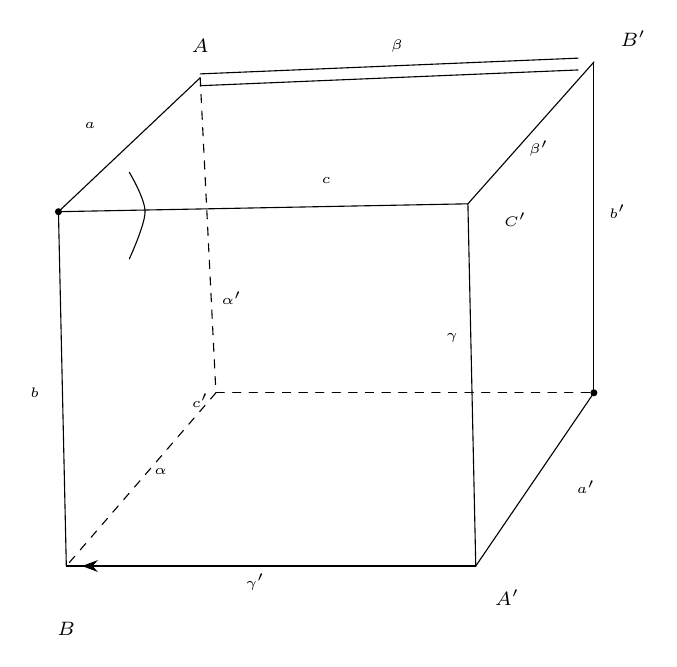
\begin{tikzpicture}[x=1mm,y=1mm,line cap=round,line join=round,font=\scriptsize]
\draw (18,-41) -- (36,-24);
\draw (18,-41) -- (70,-40);
\draw (18,-41) -- (19,-86);
\draw (70,-40) -- (71,-86);
\draw (19,-86) -- (71,-86);
\draw (70,-40) -- (86,-22);
\draw (86,-22) -- (86,-64);
\draw (71,-86) -- (86,-64);
\draw (36,-25) -- (84,-23);
\draw (36,-23.5) -- (84,-21.5);
\draw[dashed] (36,-24) -- (38,-64);
\draw[dashed] (38,-64) -- (86,-64);
\draw[dashed] (38,-64) -- (19,-86);
\node[pt] at (18,-41) {};
\node[pt] at (86,-64) {};
\draw plot[smooth, tension=0.55] coordinates {(27,-36) (29,-41) (27,-47)};
\draw[-{Stealth[length=2mm]}] (70,-86) -- (21,-86);
\node[inner sep=1pt] at (36,-20) {\scriptsize $A$};
\node[inner sep=1pt] at (61,-20) {\tiny $\beta$};
\node[inner sep=1pt] at (91,-19) {\scriptsize $B'$};
\node[inner sep=1pt] at (22,-30) {\tiny $a$};
\node[inner sep=1pt] at (52,-37) {\tiny $c$};
\node[inner sep=1pt] at (76,-42) {\tiny $C'$};
\node[inner sep=1pt] at (89,-41) {\tiny $b'$};
\node[inner sep=1pt] at (40,-52) {\tiny $\alpha'$};
\node[inner sep=1pt] at (15,-64) {\tiny $b$};
\node[inner sep=1pt] at (36,-65) {\tiny $c'$};
\node[inner sep=1pt] at (68,-57) {\tiny $\gamma$};
\node[inner sep=1pt] at (79,-33) {\tiny $\beta'$};
\node[inner sep=1pt] at (31,-74) {\tiny $\alpha$};
\node[inner sep=1pt] at (85,-76) {\tiny $a'$};
\node[inner sep=1pt] at (43,-88) {\tiny $\gamma'$};
\node[inner sep=1pt] at (19,-94) {\scriptsize $B$};
\node[inner sep=1pt] at (75,-90) {\scriptsize $A'$};
\end{tikzpicture}
\end{document}
